\documentclass[a4paper,10pt]{report}

\topmargin -2cm
%\topskip0cm
%\footskip0cm
%\headsep0cm
\parindent0cm
\oddsidemargin -1cm
\evensidemargin -1cm
\headheight 2cm
\textheight 24cm
\textwidth 18cm

\author{Daniel W\"aber (4049590)}
\title{\"Ubung}

\usepackage{ucs}
\usepackage[utf8x]{inputenc}
\usepackage{german}
\usepackage{color}
\usepackage{url}
\usepackage{graphicx}
\usepackage{algorithmic}

\pagestyle{empty}
\usepackage{makeidx}
\usepackage{amsmath}
\usepackage{amsfonts}
\usepackage{amssymb,euscript}
\usepackage{dsfont}
\usepackage{listings}
\usepackage{enumerate}
\newfont{\Fr}{eufm10}
\newfont{\Sc}{eusm10}
\newfont{\Bb}{msbm10}
\newcommand{\limin}{\lim_{n\rightarrow\infty}}
\newcommand{\limix}{\lim_{x\rightarrow\infty}}
\newcommand{\limun}{\lim_{n\rightarrow -\infty}}
\newcommand{\limux}{\lim_{n\rightarrow -\infty}}
\newcommand{\limx}{\lim_{x\rightarrow x_0}}
\newcommand{\limh}{\lim_{h\rightarrow 0}}
\newcommand{\defi}{\paragraph{Definition:}}
\newcommand{\bew}{\paragraph{Beweis:}}
\newcommand{\satz}{\paragraph{Satz:}}
\newcommand{\bsp}{\paragraph{Beispiel:}}
\newcommand{\lemma}{\paragraph{Lemma:}}
\newcommand{\N}{\mathds{N}}
\newcommand{\F}{\mathds{F}}
\newcommand{\Z}{\mathds{Z}}
\newcommand{\Q}{\mathds{Q}}
\newcommand{\R}{\mathds{R}}
\newcommand{\G}{\mathds{G}}
\newcommand{\C}{\mathds{C}}
\newcommand{\K}{\mathds{K}}
\newcommand{\A}{\mathds{A}}
\newcommand{\E}{\mathcal{E}}
\renewcommand{\P}{\mathcal{P}}
\newcommand{\sigA}{$\sigma$-Algebra }
\newcommand{\qed}{$\hfill\blacksquare$}
\newcommand{\arsinh}{\operatorname{arsinh} }
\newcommand{\arcosh}{\operatorname{arcosh} }
\newcommand{\gdw}{ $ \Leftrightarrow $ }
\newcommand{\tf}{ $ \Rightarrow $ }
\newcommand{\mgdw}{\Leftrightarrow}
\newcommand{\mtf}{\Rightarrow}
\newcommand{\Bild}{\text{Bild}}
\newcommand{\Kern}{\text{kern}}
\newcommand{\rg}{\text{rg}}
\newcommand{\deff}{\text{deff}}

\newcommand{\alphato}{\underset{\alpha}\to}
\newcommand{\betato}{\underset{\beta}\to}
\newcommand{\etato}{\underset{\eta}\to}
\newcommand{\ito}{\underset{i}\to}
\newcommand{\sto}{\underset{s}\to}
\newcommand{\kto}{\underset{k}\to}
\newcommand{\xto}{\underset{x}\to}

\usepackage{fancyhdr}
\pagestyle{fancy}
\lhead{Daniel Waeber\\Alex Muenn}
\chead{"Ubungsblatt \nr\\\today}
\rhead{Bildverarbeitung}


\newcommand{\nr}{10}
\lstset{language=matlab}

\begin{document}
\section*{Aufgabe 1 - Hough-Transformation - Geradenerkennung}

Ausgangsbild war ``street'', was wir f\"ur einfachere Weiterverarbeitung
auf eine Zweierpotenz skalierten und entsprechend wei\ss{}/graue Balken
erweiterten.
\begin{figure}[H]
\begin{center}
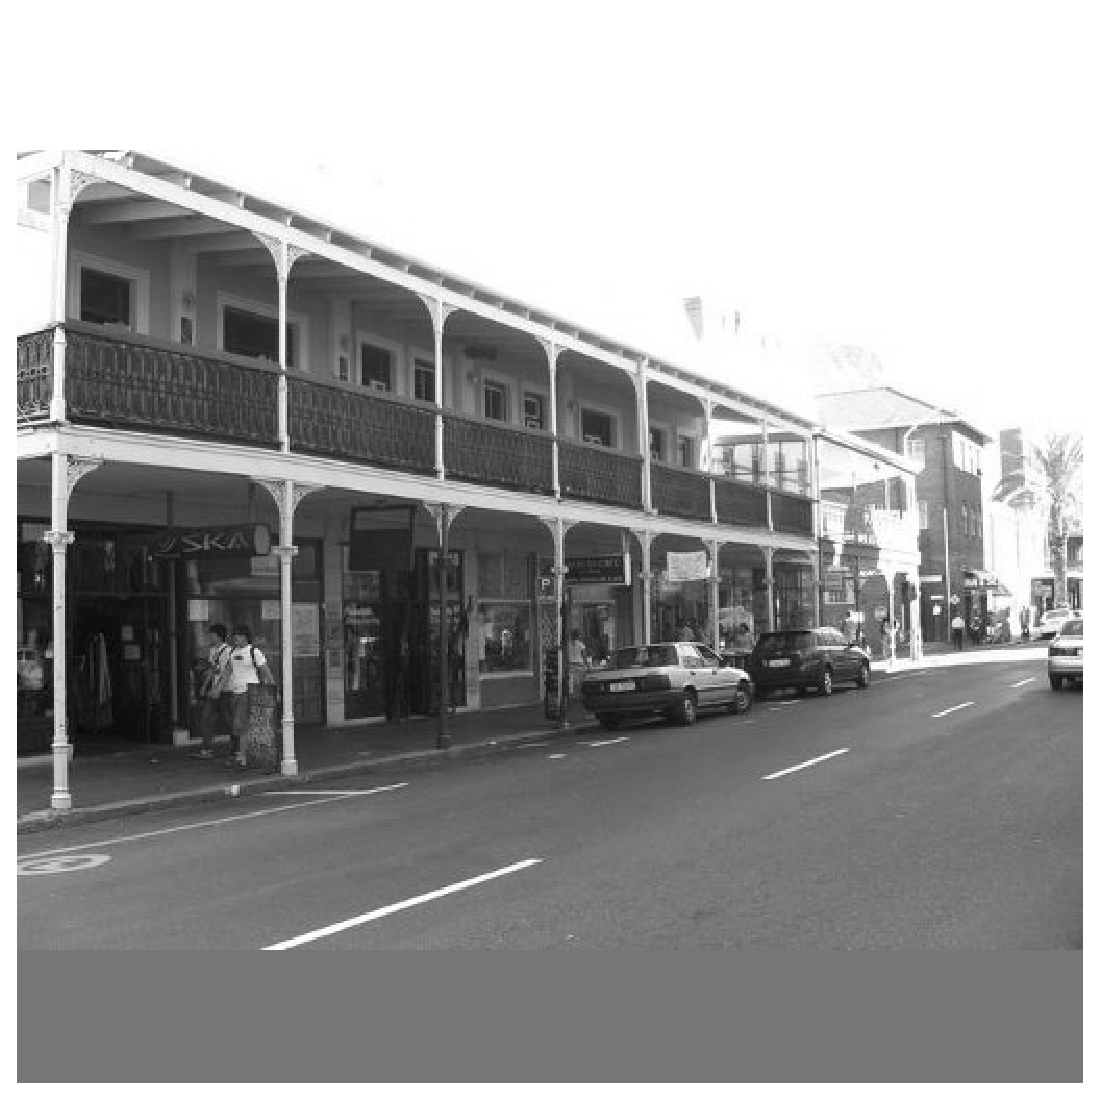
\includegraphics[width=100mm]{u10/street.eps}
\end{center}
\label{street}
\caption{Street - Ausgangsbild}
\end{figure}

Davon ausgehend f\"uhrten wir eine Vorverarbeitung durch. Aus vorhergehenden
U\"bungen verwendeten wir Ableitung nach X- und Y-Richtung (Soebel), berechneten 
den Gradienten (Polarkoordinaten). Zus\"tzlich binarisierten wir das Ergebnis der Gradientenberechnung,
um nur relevante Pixel in die Betrachtung als potentielle Teile einflie\ss{}en zu lassen.

\begin{figure}[H]
\begin{center}
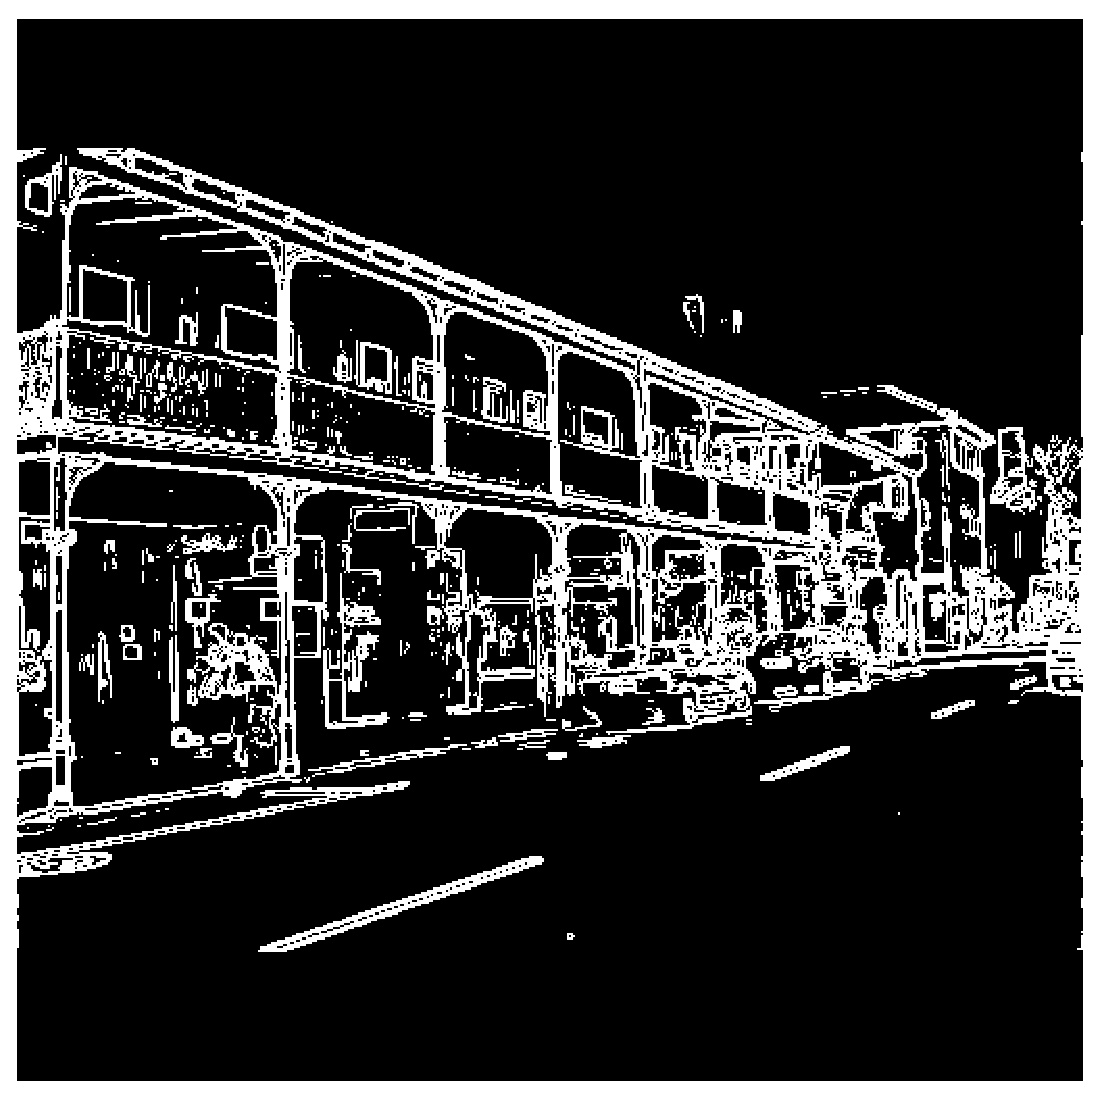
\includegraphics[width=100mm]{u10/street_edges.eps}
\end{center}
\label{streete}
\caption{Nur die Gradienten der wei\ss en Pixel werden betrachtet}
\end{figure}

Im letzten Schritte verwendeten wir den Algorithmus aus der Vorlesung, bei dem 
m\"ogliche Geradenverl\"aufe in Abh\"angigkeit von $d = x \cdot \cos \teta  + y \cdot \sin \teta $
betrachtet werden. $\Teta$ geht aus der Gradientenrichtung hervor plus einem zus\"atzlichen
Abweichungsfenster. Die Werte werden diskretisiert und in eine Matrix gespeichert. Die Visualisierung
der Matrix sieht dann wie folgt aus:

\begin{figure} [H]
\begin{center}

\includegraphics[width=100mm]{u10/street_lines.eps}
\end{center}
\label{streetl}
\caption{Die erkannten Geraden}
\end{figure}

Interpretation der Grafik: Abbildung von $d$ auf $\teta$, wobei der Nullpunkt in der linken oberen
Ecke liegt. Der Wertebereich von $\teta$ l\"auft von $-\pi$ bis $+\pi$. Zu erkennen sind zwei 
wesentliche Geradenarten. Die mit Variationen um die null Grad und steigendem Abstand (also 
horizontale Linien, die perspektivisch verlaufen) und die Senkrechten, die im geringen Abstandsbereich
dominieren (weil sie auch fl\"achenm\"assig \"uberwiegen) aber in einem konstanten Winkel (90 Grad)
verlaufen.
\\
Anmerkung: W\"ahrend der Erstellung der Matrix mussten wir mehrmals (durch probieren) die
Interpretation der Werte \"andern. Um negative Ds zum Beipsiel zu vermeiden, ist es n\"otig
den Komplementwinkel zu verwenden, wenn nur der Betrag von D verwendet werden soll.

\section*{Aufgabe 2 - Kreiserkennung}
\ldots


\end{document}
